% Chapter Analysis Strategy

\chapter{Systematic Uncertainty} \label{Sysyematic Uncertainty}

\section{Systematic Uncertainty on Signal Selection} \label{Event reconstruction and selection}

\begin{itemize}
%CMS-PAS-LUM-17-001
  \item Luminosity: Intergrated luminosity is estimated with 2.5$\% $ uncertainty. 
  \item Pile-ups: Pile-up efficiecny scale factor is applied to simulation weight the pile-up distribution as that of data. The pile-up distribution of data is measured by assuming minibias cross section equals to 69.2 mb, which has 4.6$\% $ uncertainty. 
\begin{figure}[t]
  \centering
 \begin{tabular}{cc}
    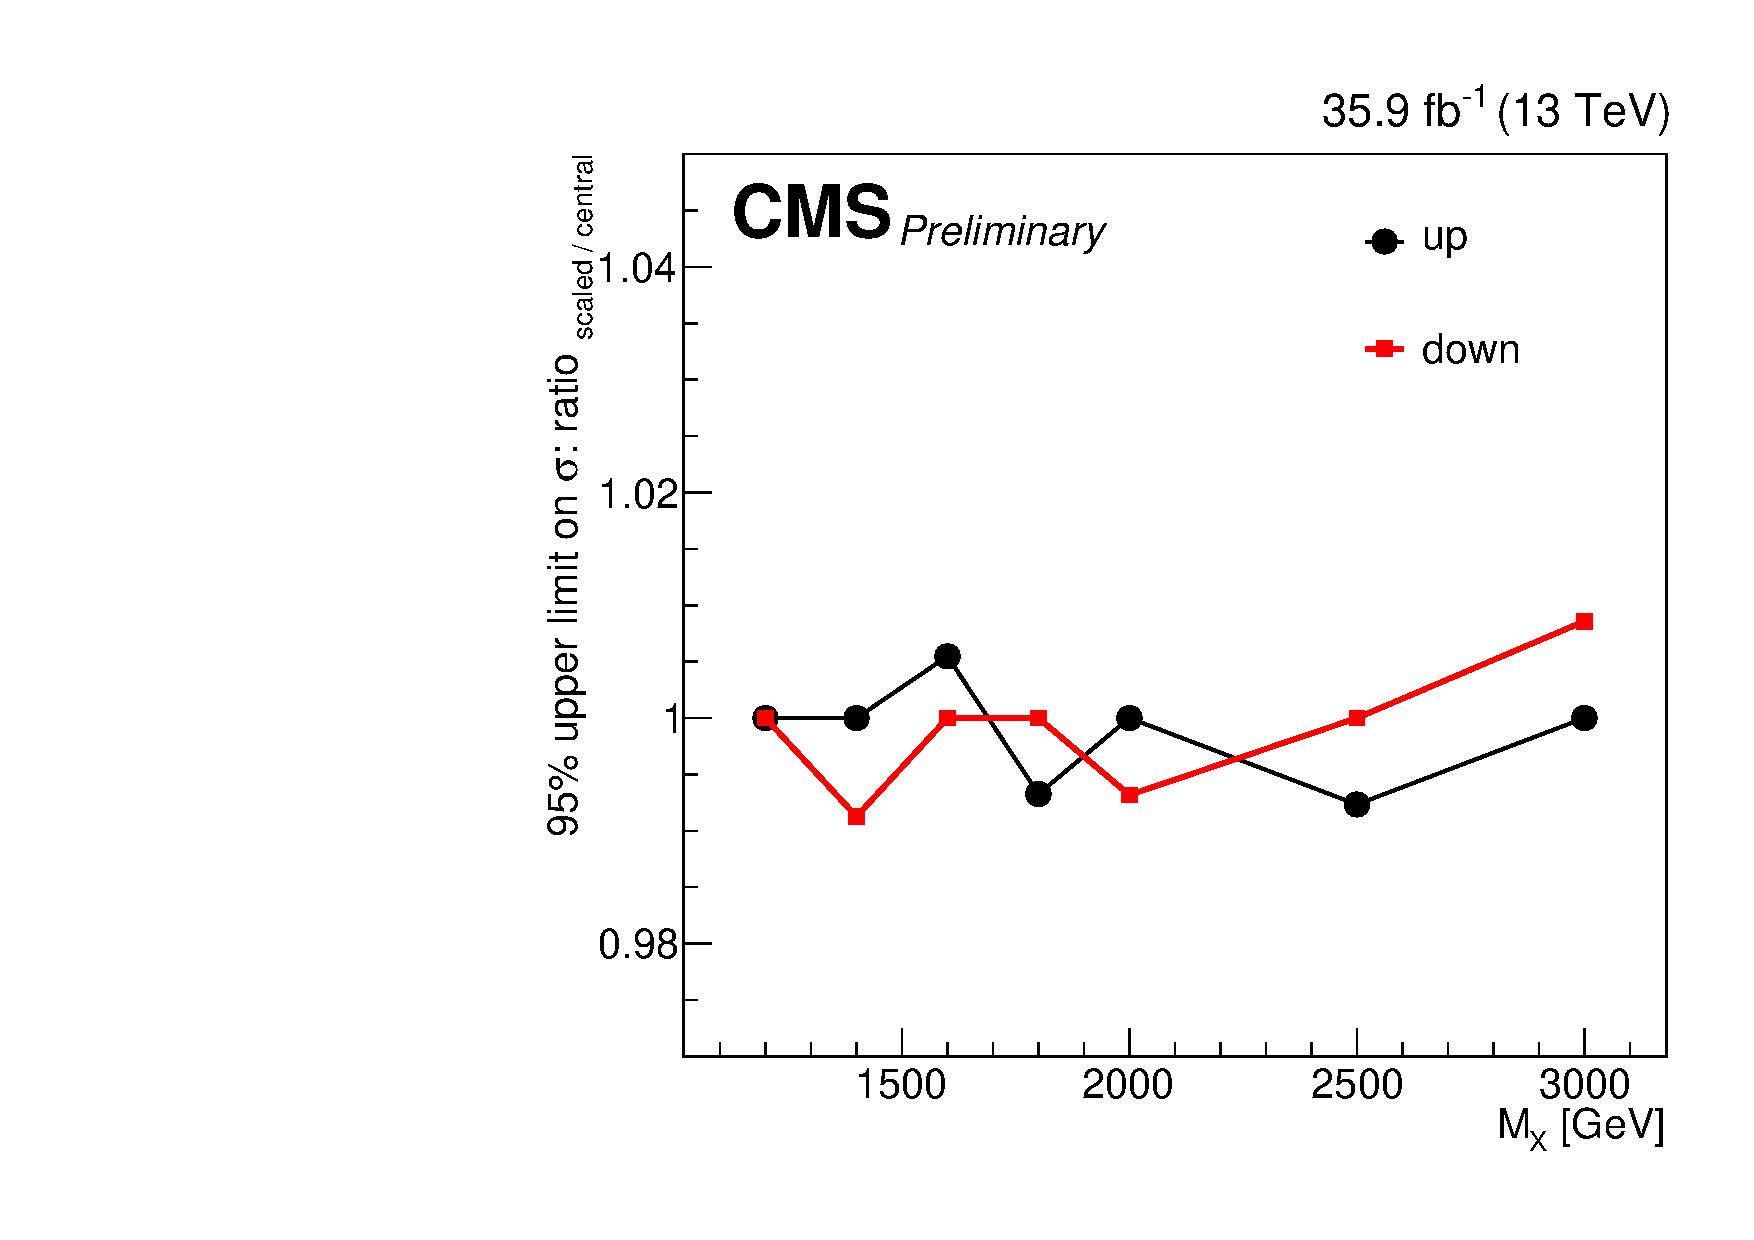
\includegraphics[width=0.5\textwidth]{Figures/plots_uncert/pu_TT.pdf} &
   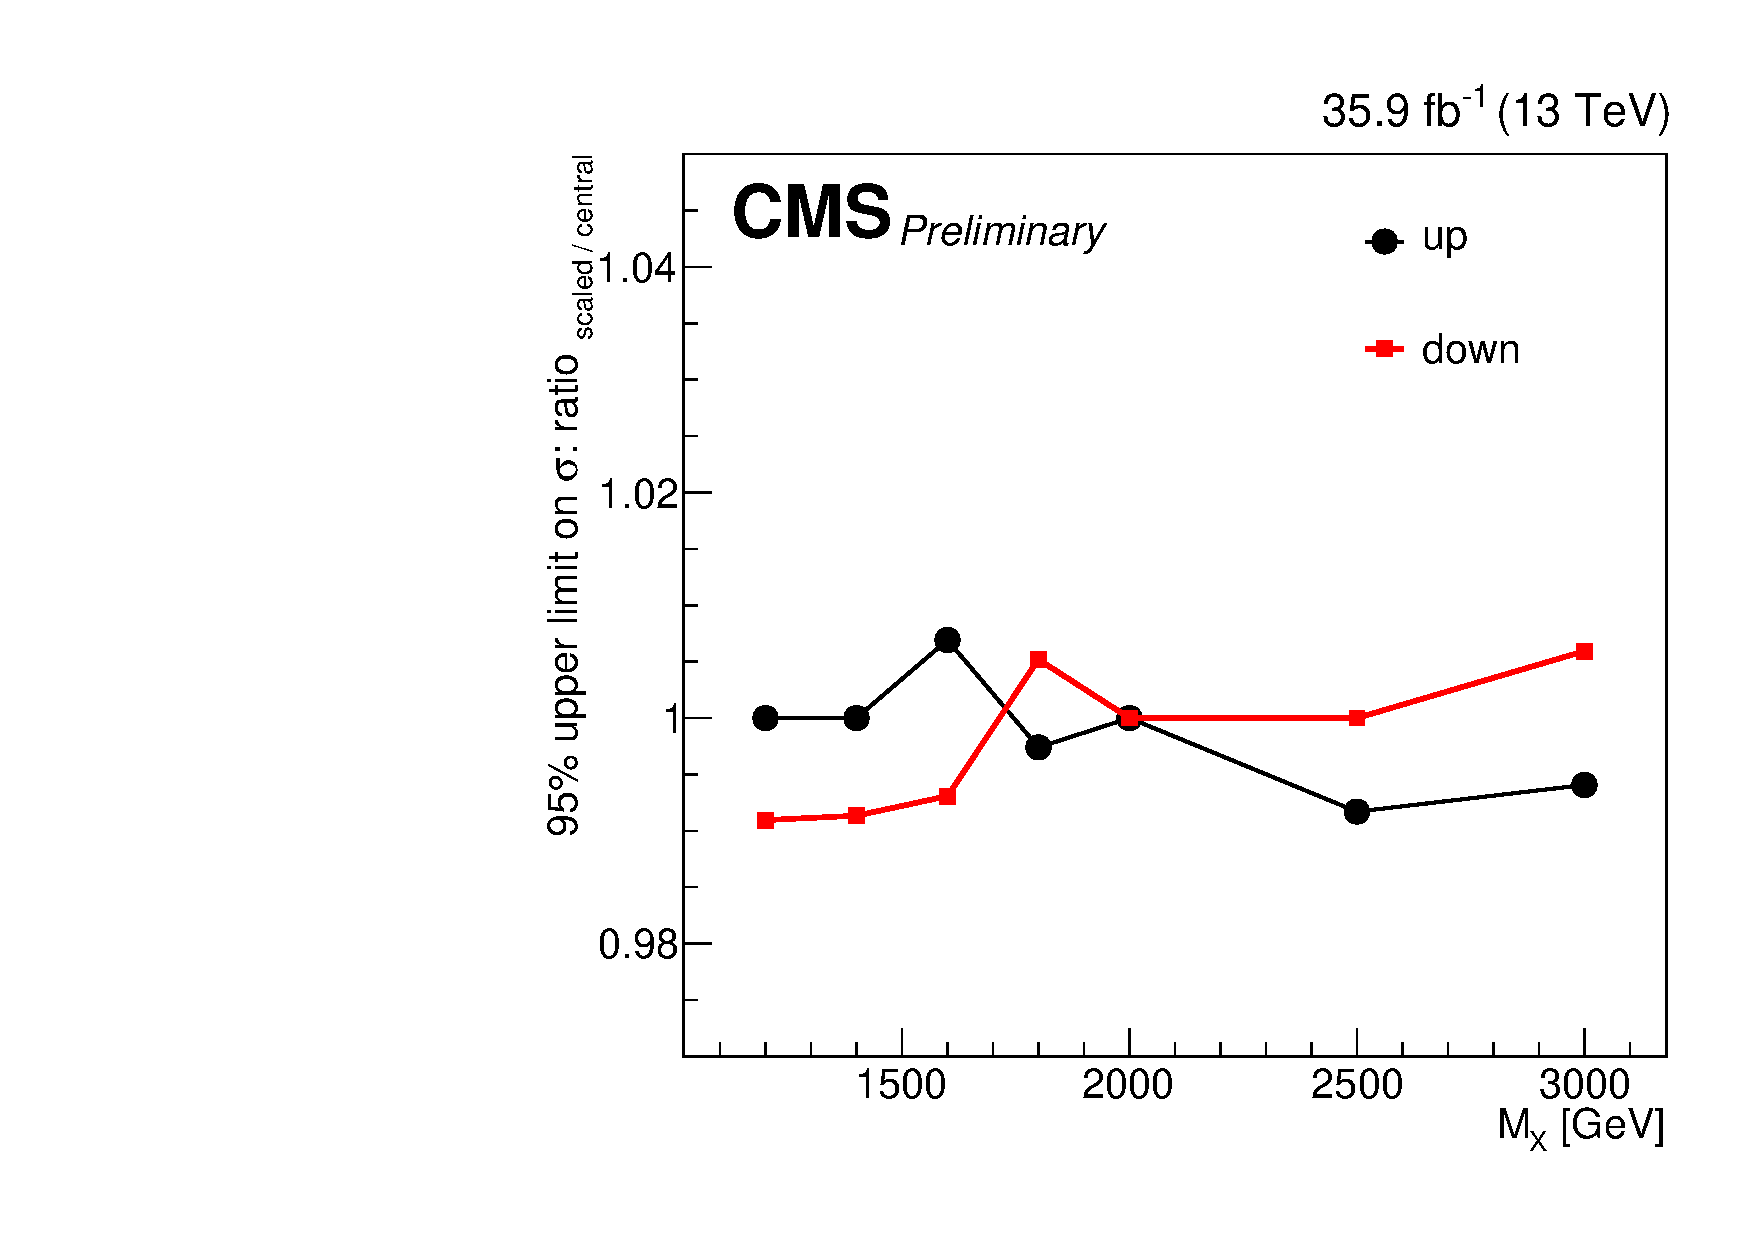
\includegraphics[width=0.5\textwidth]{Figures/plots_uncert/pu_LL.pdf} \\
  \end{tabular}
  \caption{The pile-up uncertainty. The scale-up and scale-down to central ratio based on the change of the upper limit are shown in TT (left) and LL (right) category.}
  \label{fig:hvt_brs}
\end{figure}  
   
  \item Double-b tagger scale factor:
  
\begin{figure}[t]
  \centering
 \begin{tabular}{cc}
    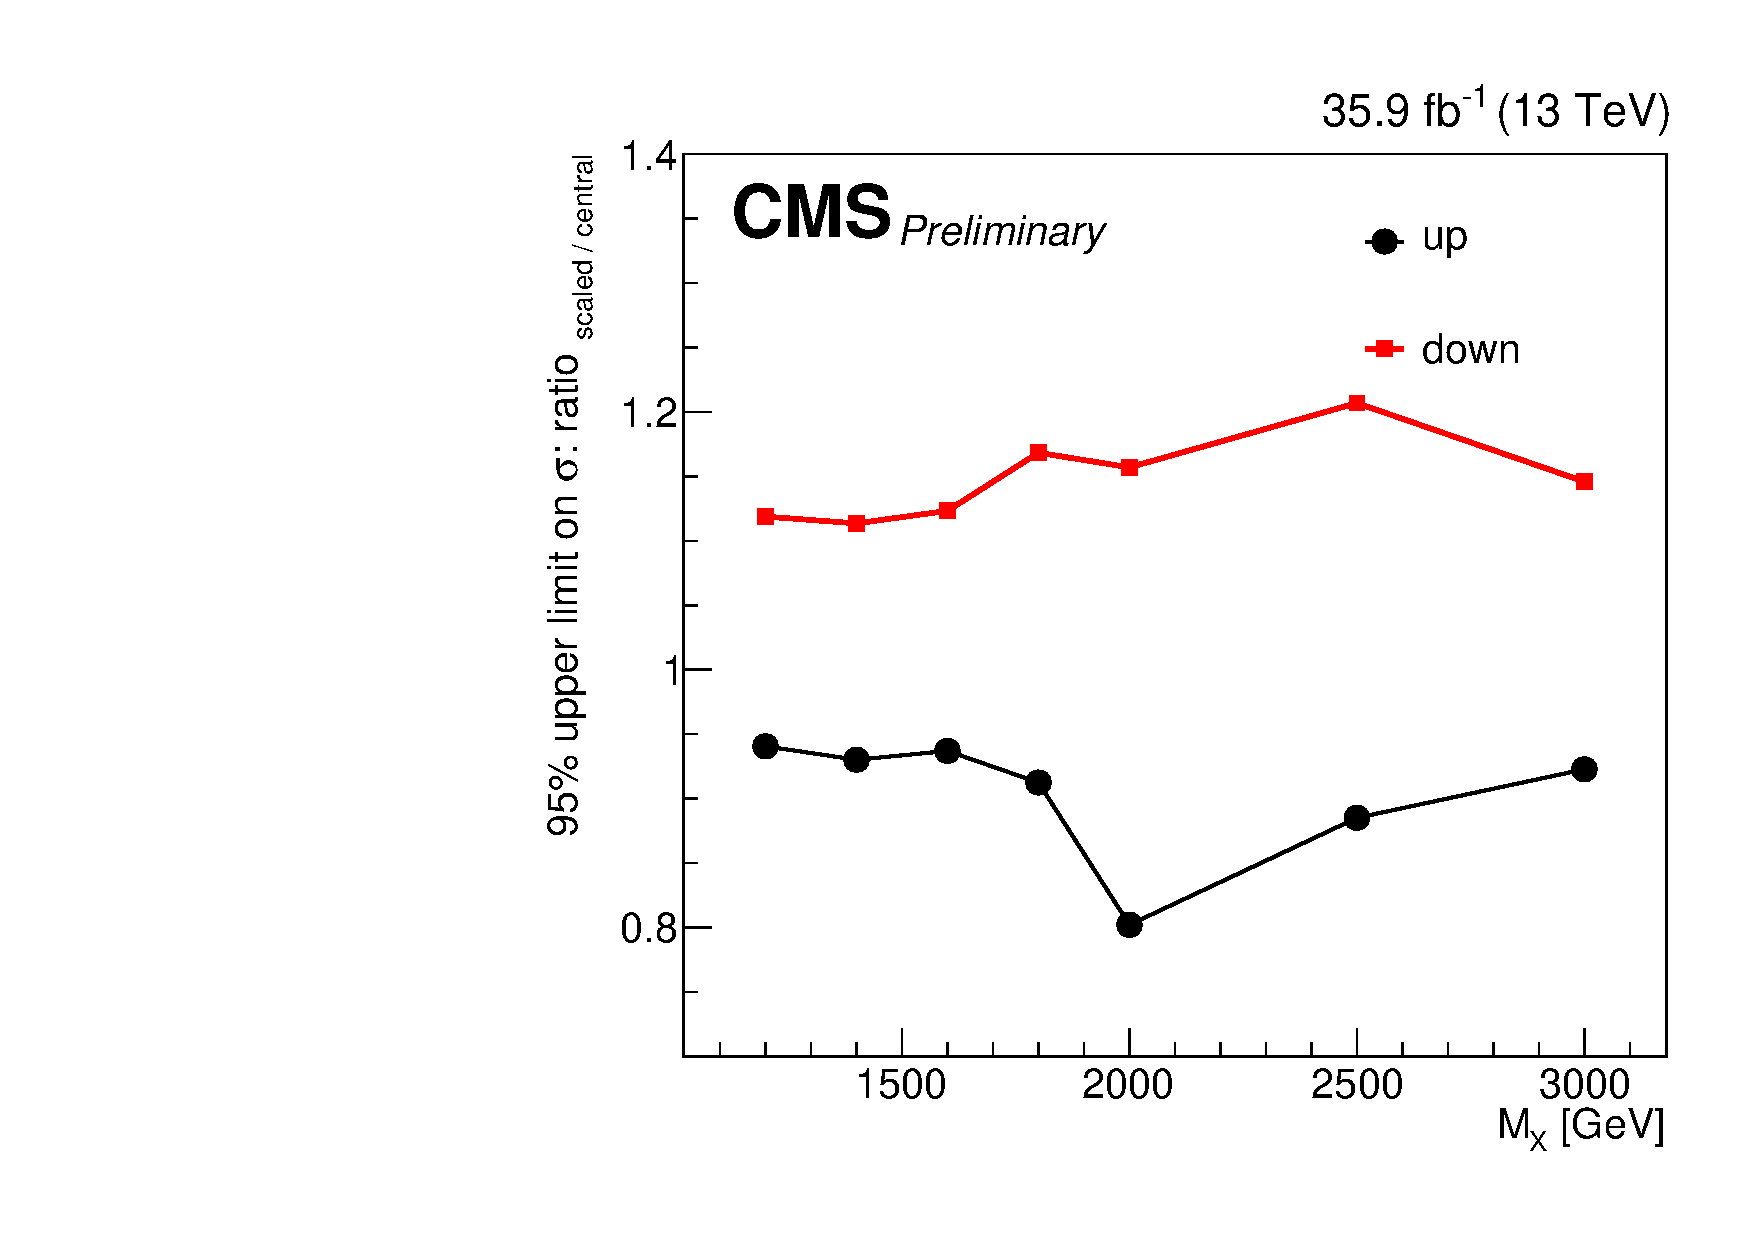
\includegraphics[width=0.5\textwidth]{Figures/plots_uncert/btag_TT.pdf} &
   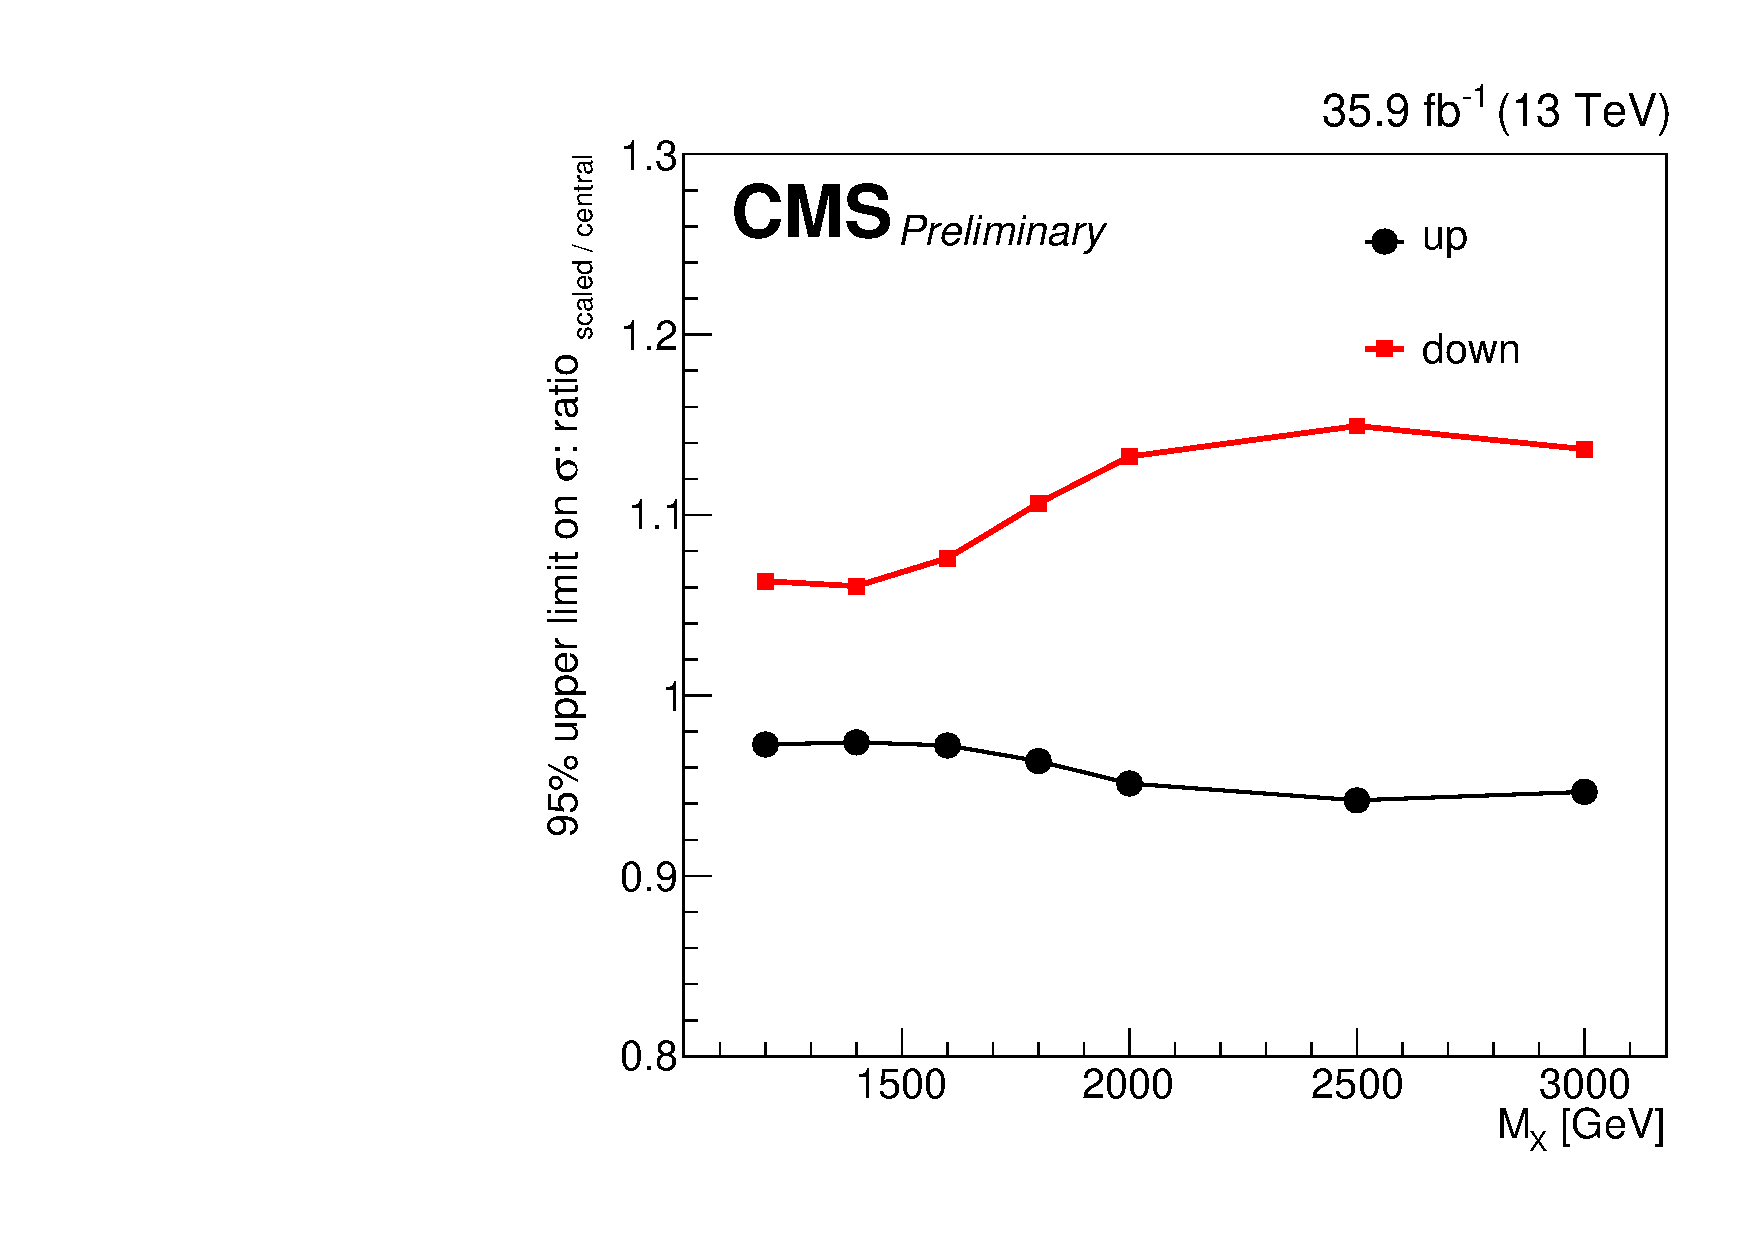
\includegraphics[width=0.5\textwidth]{Figures/plots_uncert/btag_LL.pdf} \\
  \end{tabular}
  \caption{The double-b tagger uncertainty. The scale-up and scale-down to central ratio based on the change of the upper limit are shown in TT (left) and LL (right) category.}
  \label{fig:hvt_brs}
\end{figure}    
  
%https://twiki.cern.ch/twiki/bin/viewauth/CMS/JetWtagging
  \item $\tau _{21}$ scale factor: The uncertainty of $\tau _{21}$ scale factor is measured by JME POG on the samples of semi-leptonic $t\bar{t}$ which is a generous source of W boson. The uncertainty of scale factor in the region $\tau _{21} <$ 0.55 is 14$\% $ per jet.
 
%https://twiki.cern.ch/twiki/bin/view/CMS/JetResolution#Smearing_procedures 
  \item Jet energy resoultion: The procedure is to smear the energy resolution of AK8 jets of simulation as same as those of data.  
  
  \begin{figure}[t]
  \centering
 \begin{tabular}{cc}
    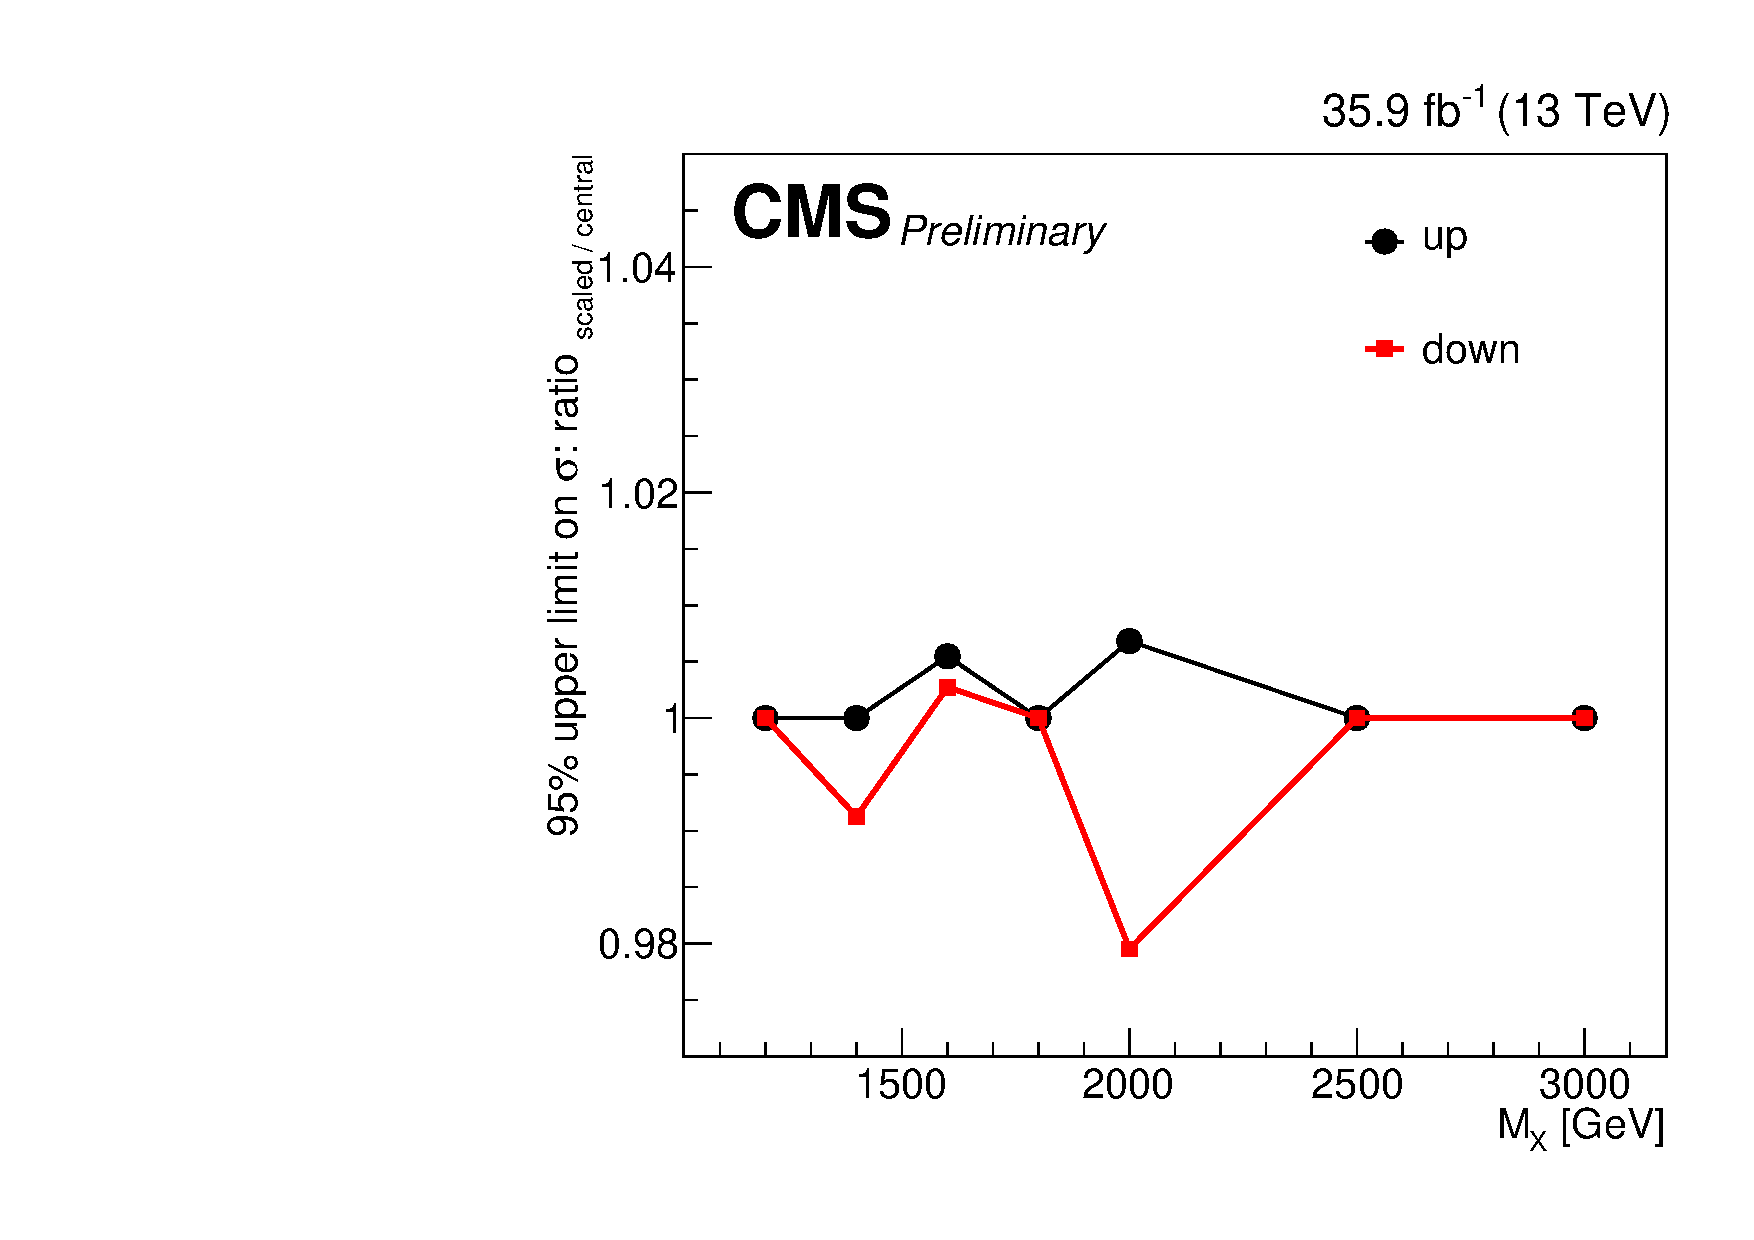
\includegraphics[width=0.5\textwidth]{Figures/plots_uncert/JER_TT.pdf} &
   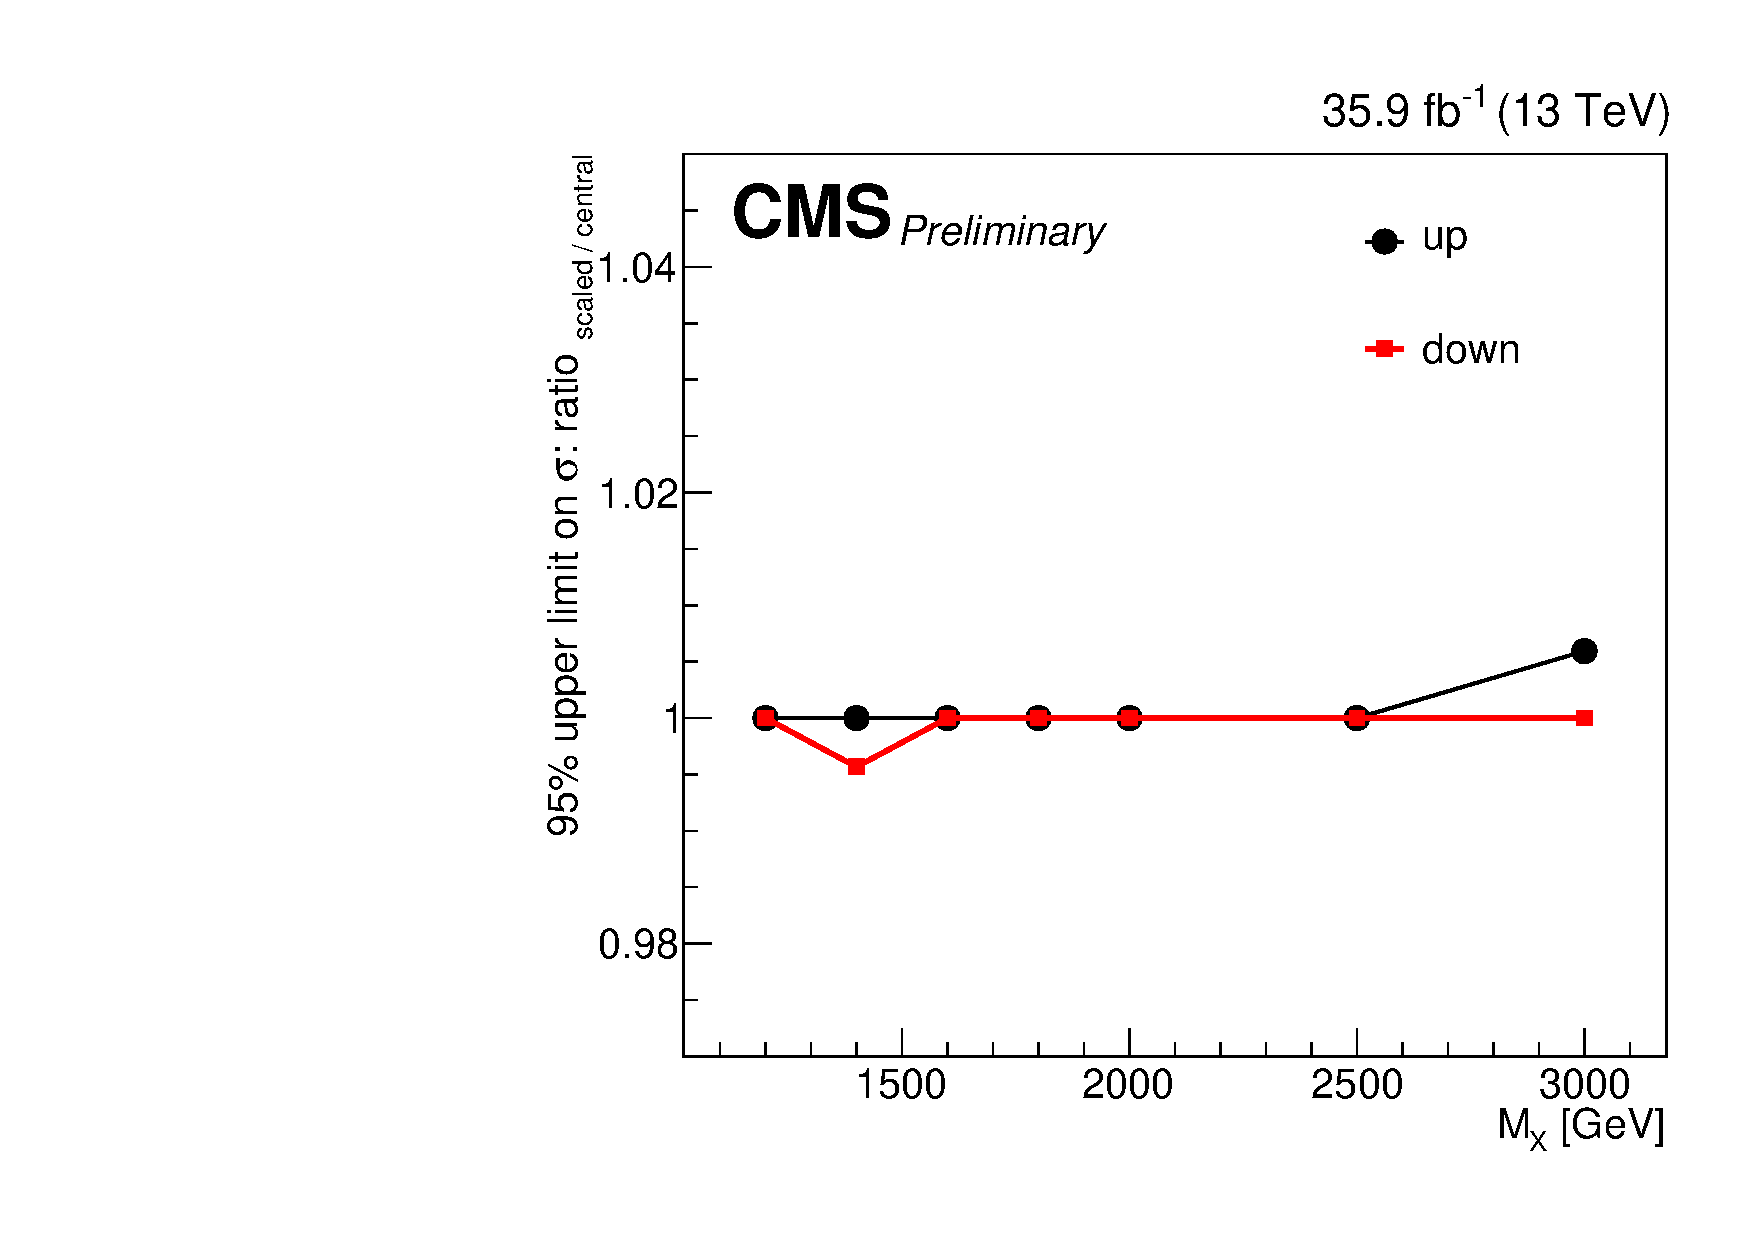
\includegraphics[width=0.5\textwidth]{Figures/plots_uncert/JER_LL.pdf} \\
  \end{tabular}
  \caption{The jet energy resoultion uncertainty. The scale-up and scale-down to central ratio based on the change of the upper limit are shown in TT (left) and LL (right) category.}
  \label{fig:hvt_brs}
\end{figure}  
  \item Jet energy scale:
  
  \begin{figure}[t]
  \centering
 \begin{tabular}{cc}
    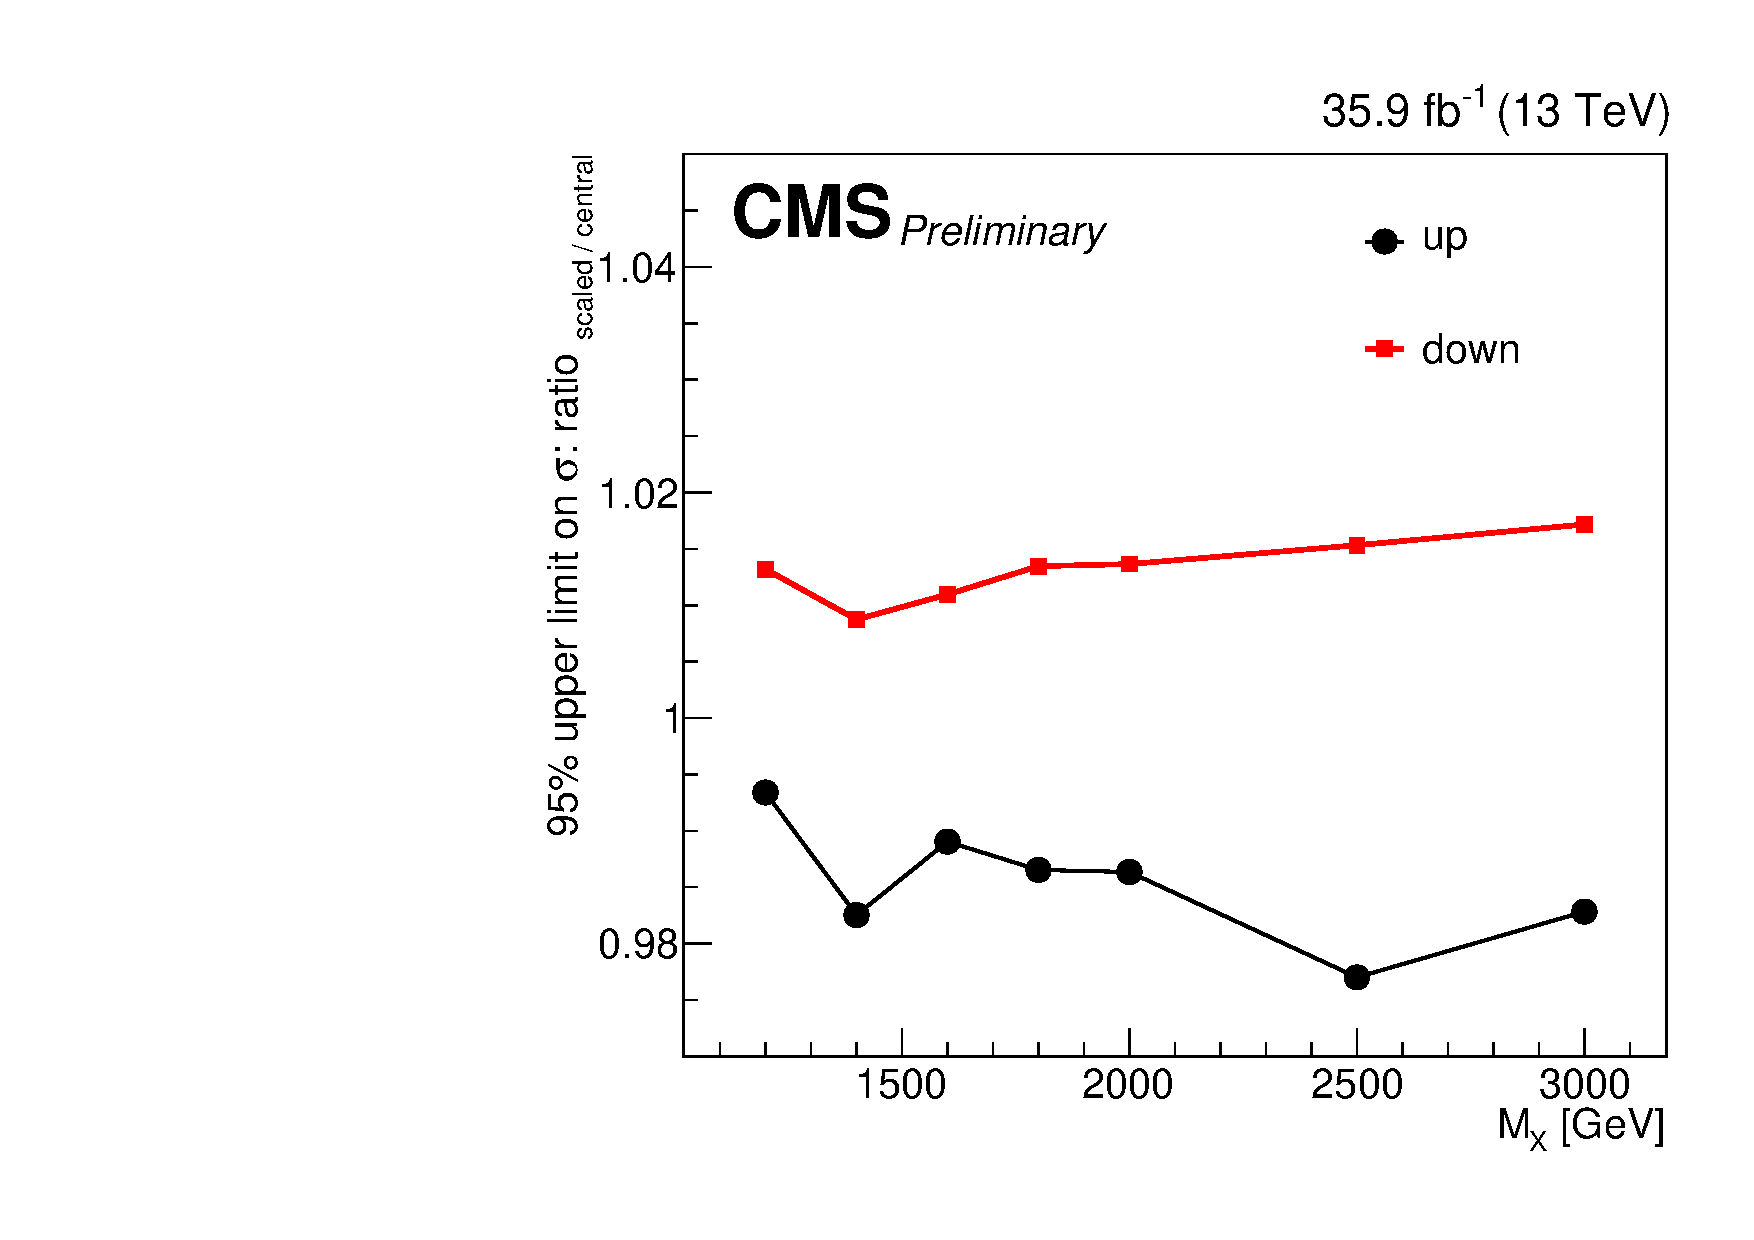
\includegraphics[width=0.5\textwidth]{Figures/plots_uncert/JEC_TT.pdf} &
   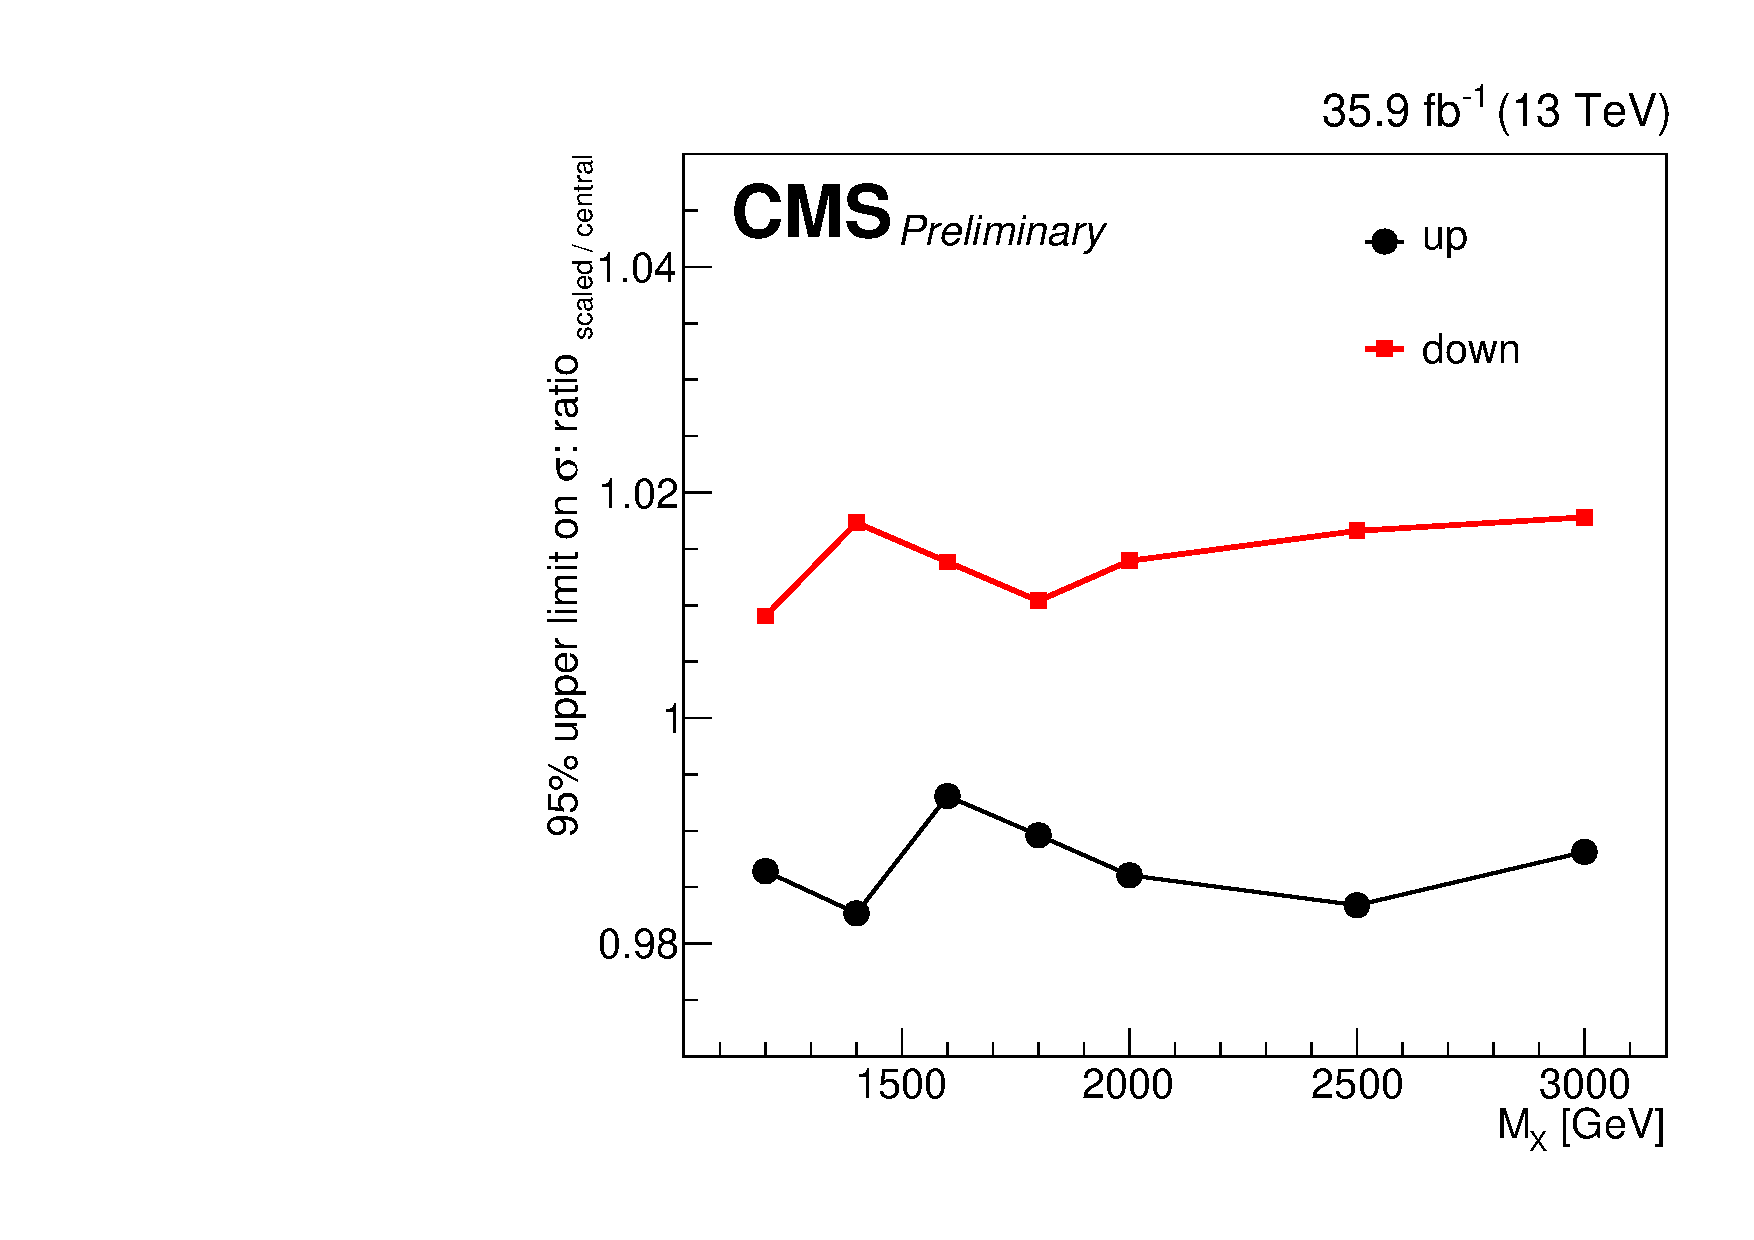
\includegraphics[width=0.5\textwidth]{Figures/plots_uncert/JEC_LL.pdf} \\
  \end{tabular}
  \caption{The jet energy scale uncertainty. The scale-up and scale-down to central ratio based on the change of the upper limit are shown in TT (left) and LL (right) category.}
  \label{fig:hvt_brs}
\end{figure} 

 \begin{figure}[t]
  \centering
 \begin{tabular}{cc}
    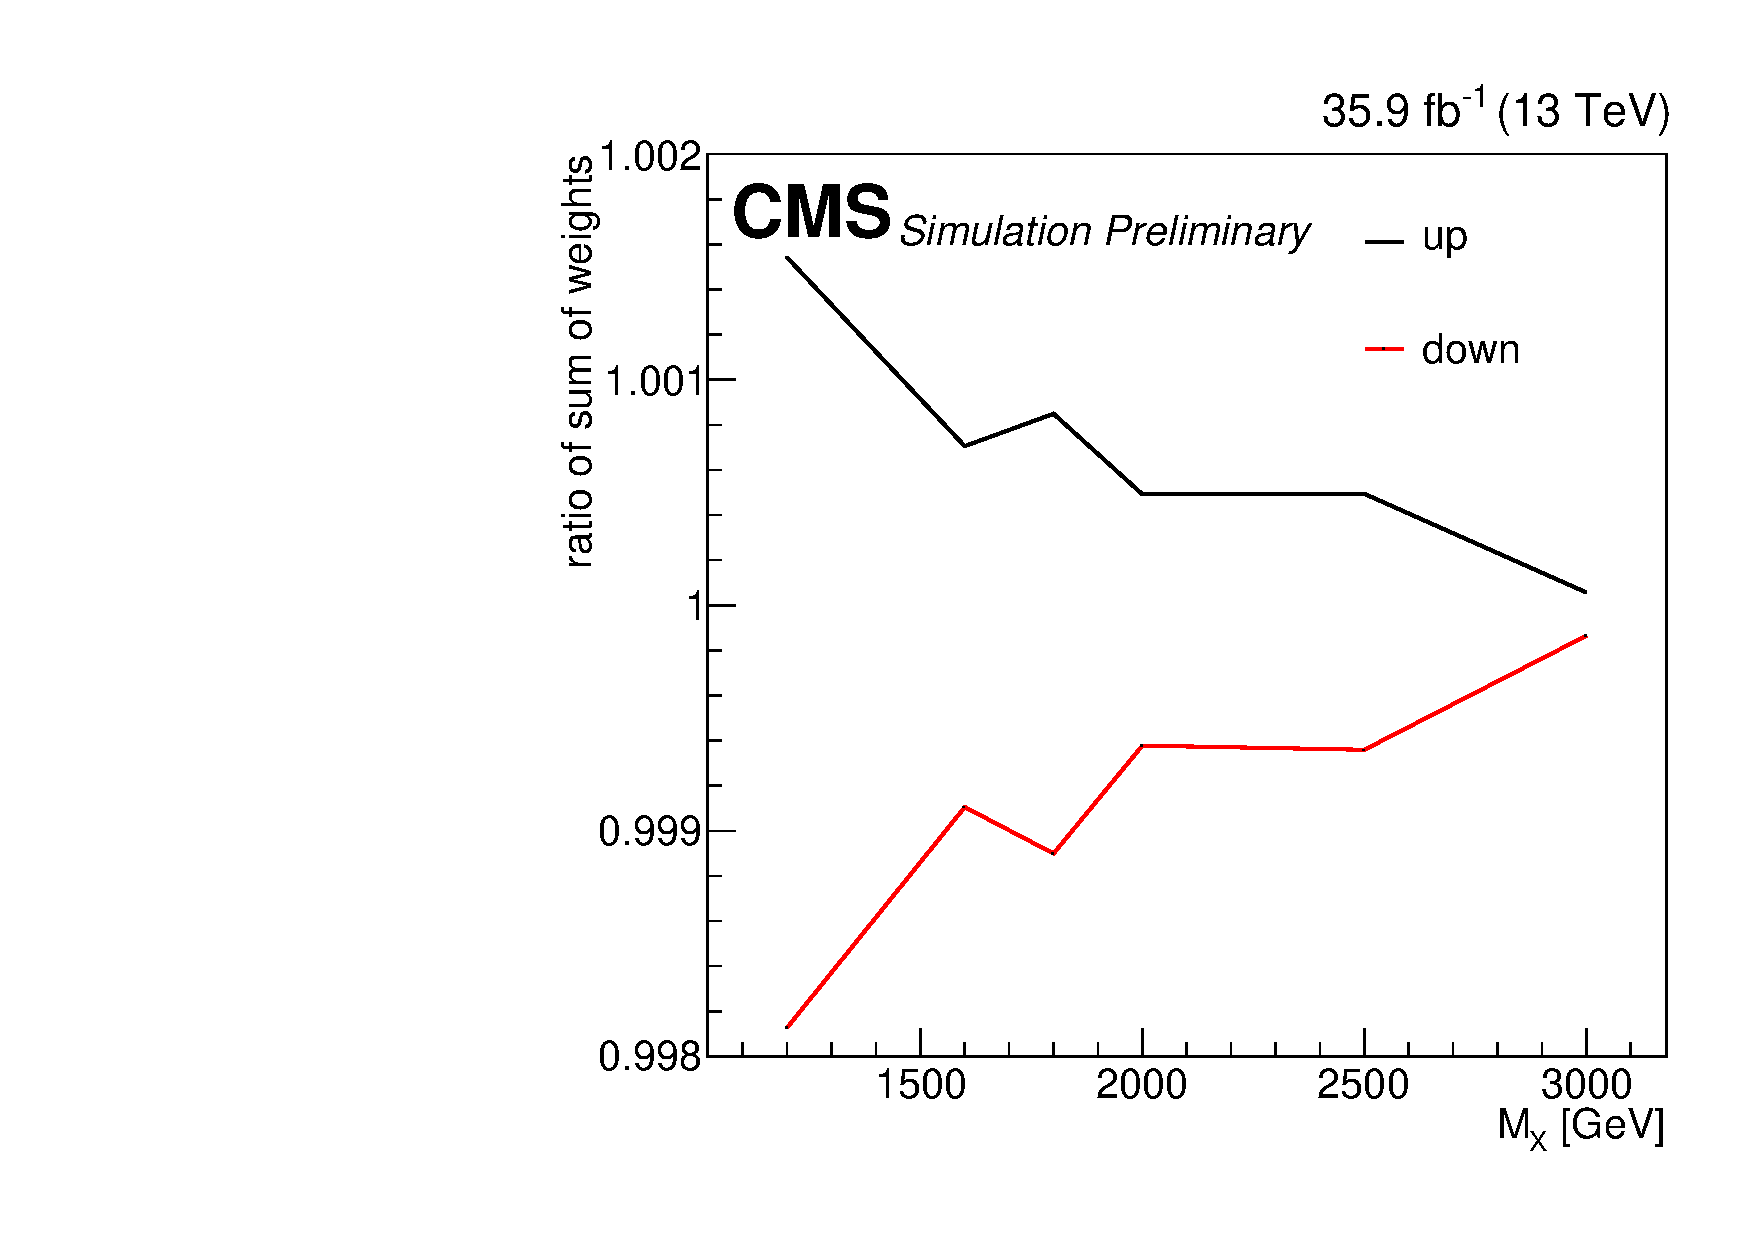
\includegraphics[width=0.5\textwidth]{Figures/scl/scl_TT.pdf} &
   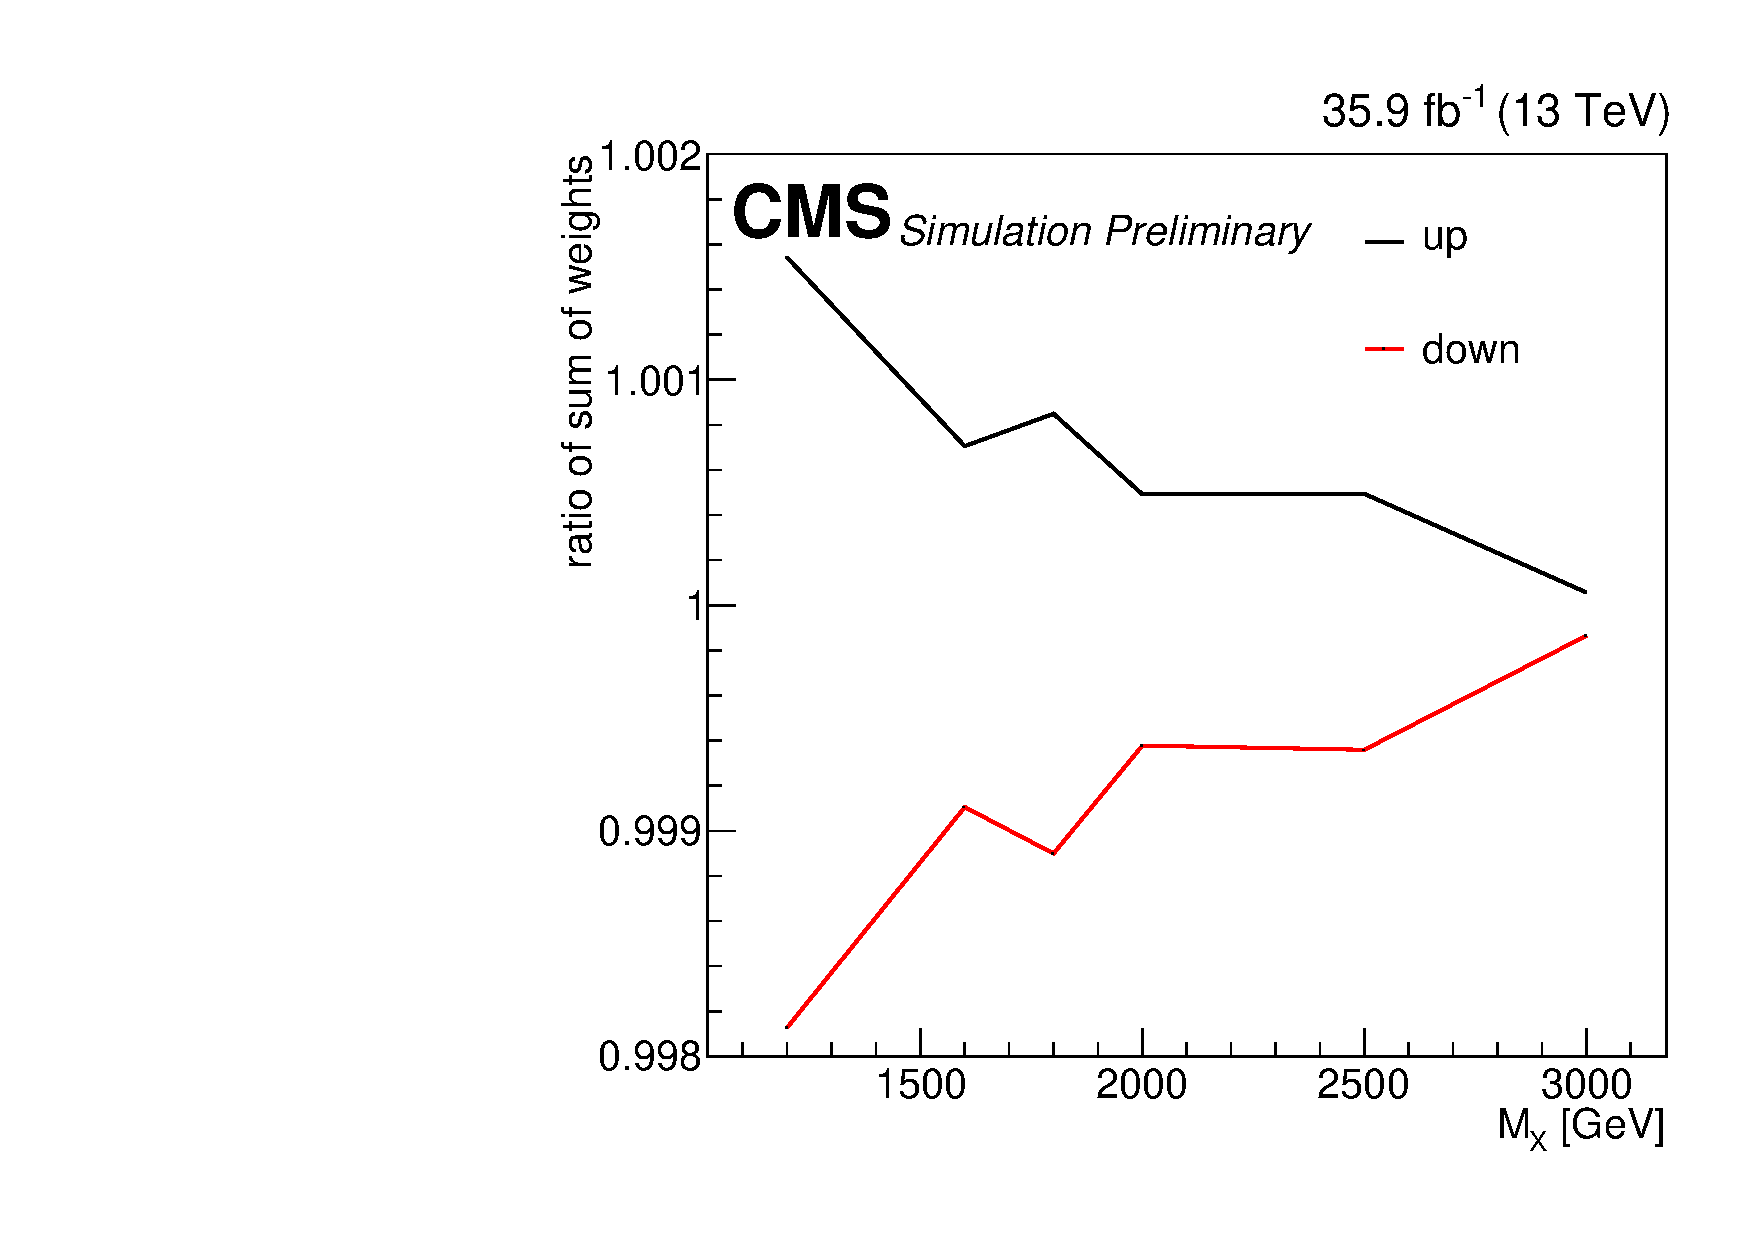
\includegraphics[width=0.5\textwidth]{Figures/scl/scl_TT.pdf} \\
  \end{tabular}
  \caption{The Factorization uncertainty. The scale-up and scale-down to central ratio based on the change of the efficiecny are shown in TT (left) and LL (right) category.}
  \label{fig:hvt_brs}
\end{figure} 

 \begin{figure}[t]
  \centering
 \begin{tabular}{cc}
    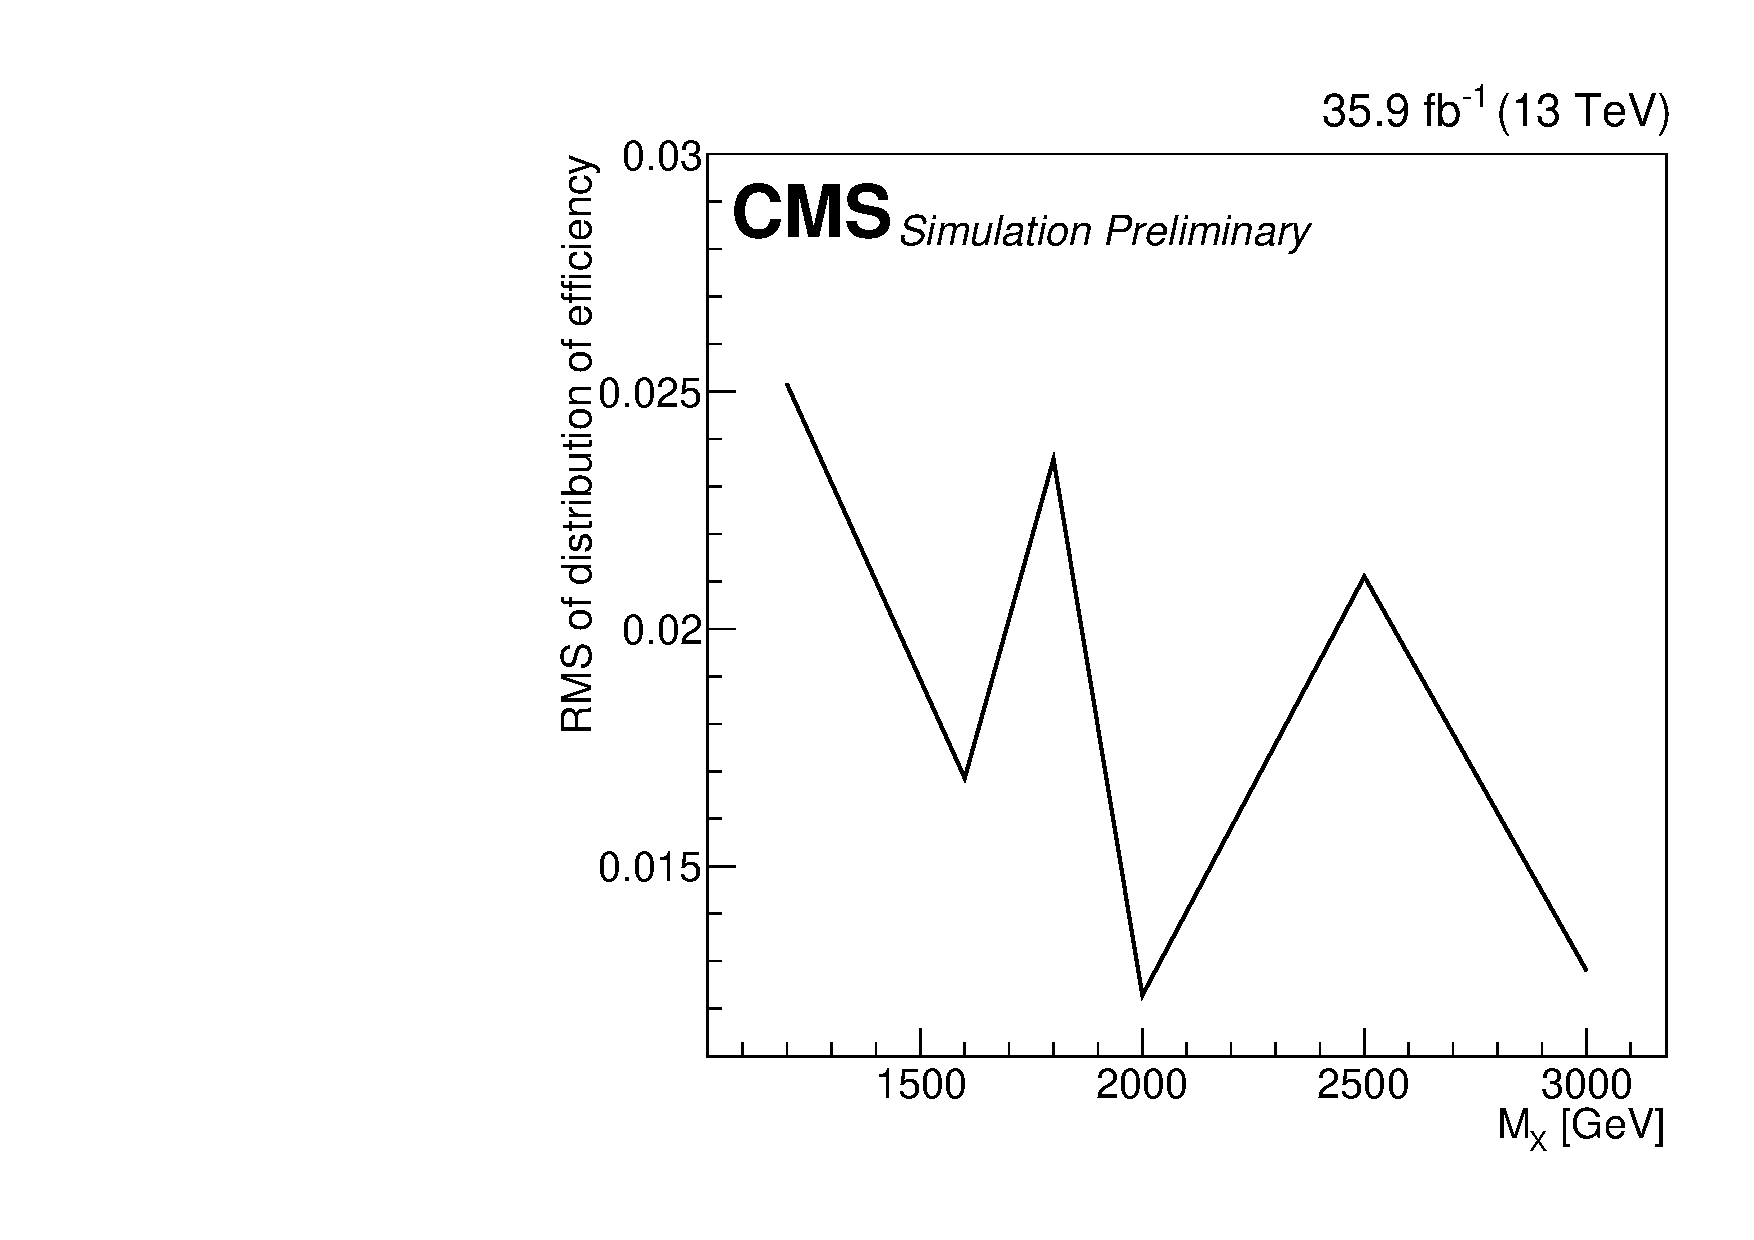
\includegraphics[width=0.5\textwidth]{Figures/eff/uncert_pdf_eff_TT.pdf} &
   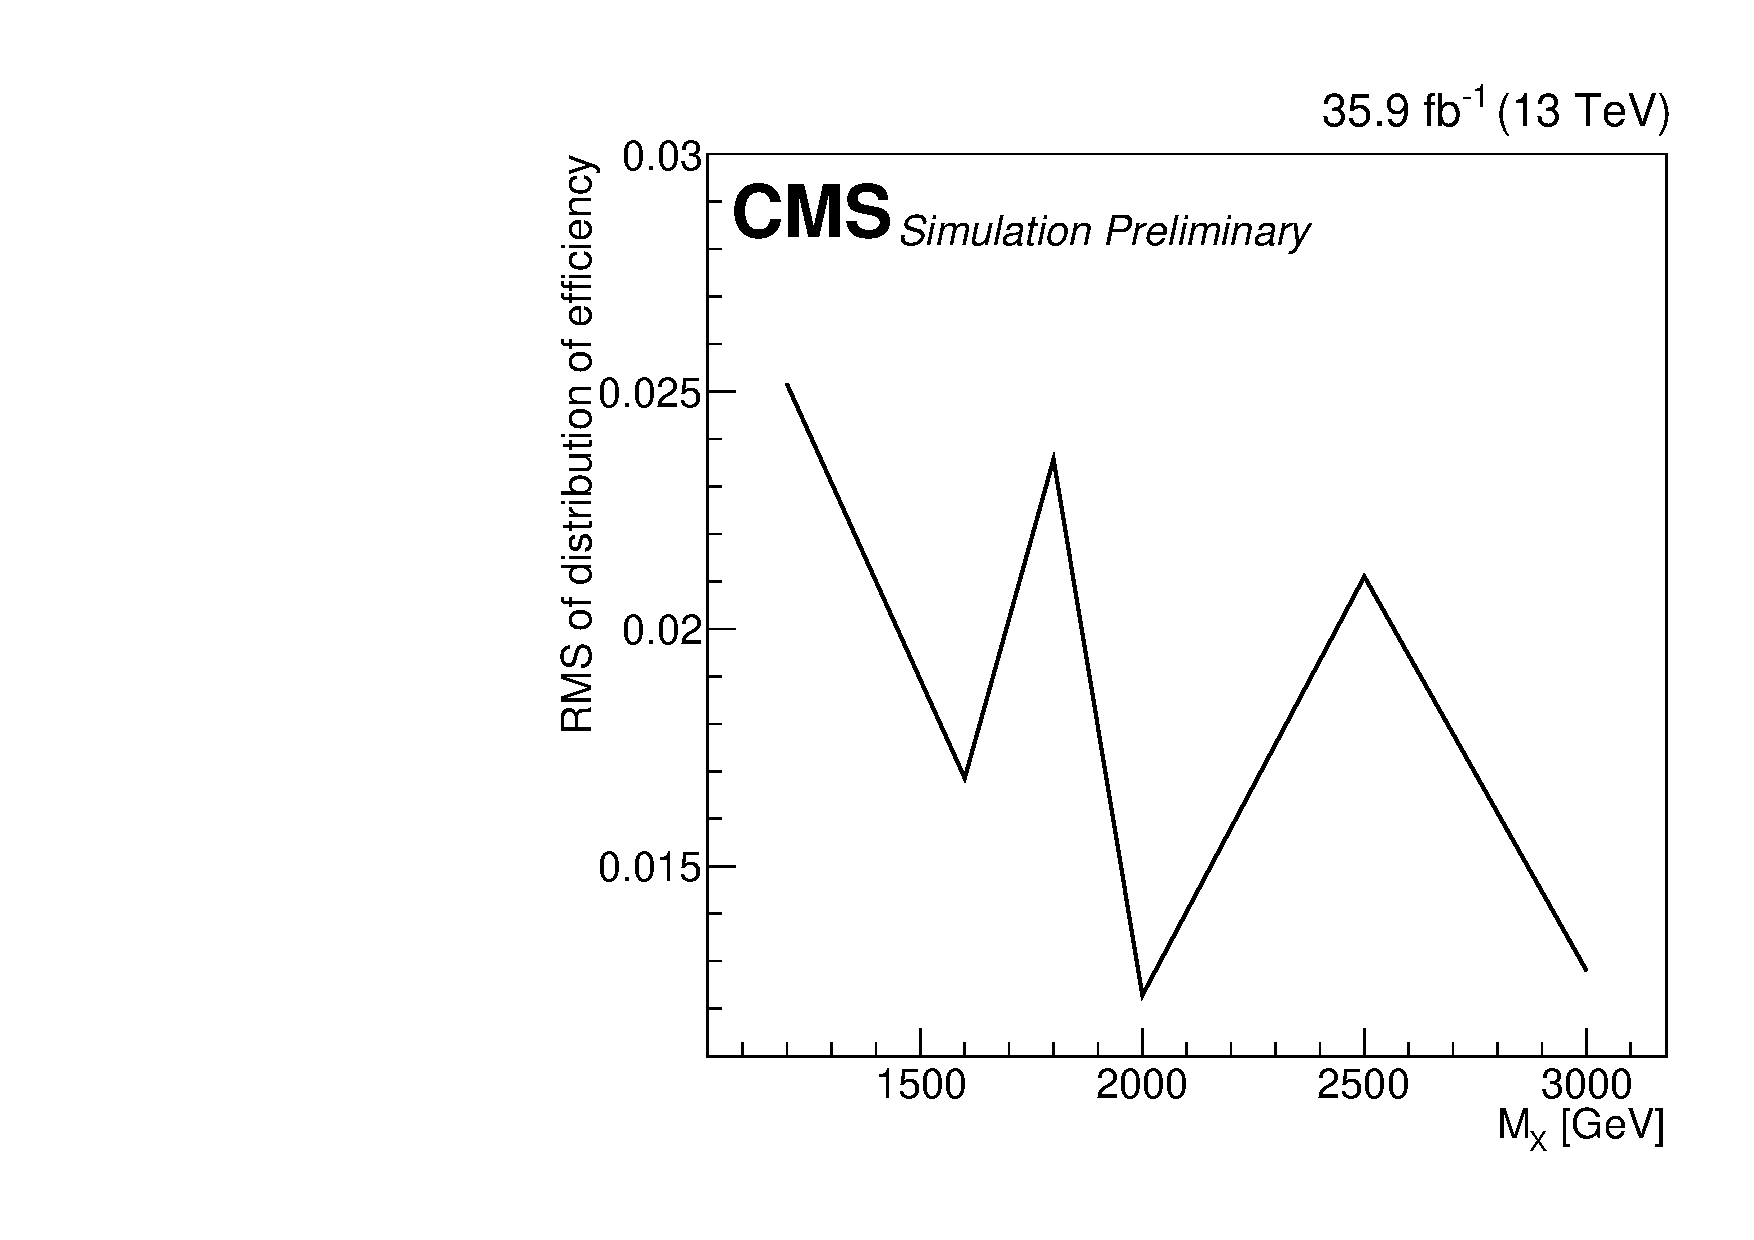
\includegraphics[width=0.5\textwidth]{Figures/eff/uncert_pdf_eff_TT.pdf} \\
  \end{tabular}
  \caption{The jet energy scale uncertainty. The values of ratio RMS of efficiecny from 100 p.d.f. sets to efficiecny of central value are shown in TT (left) and LL (right) category.}
  \label{fig:hvt_brs}
\end{figure}  

	\item Trigger efficiency scale factor: the trigger efficiency scale factor is measured by the ratio of the efficiency of simulation to that of data. Since we veto the leptonic events, we use JetHt dataset instead of Single-muon dataset to measure the efficiency of data. The pre-selection is listed:
   \begin{itemize}
	\item Two leading AK8 jets have $p_{T} >$ 300 GeV and |$\eta$| $<$2.4.
	\item 105 $<$ corrected PUPPI soft-drop maas $<$ 135.
	\item $\Delta \eta$(two leading AK8 jets) $<$ 1.3.
	\end{itemize}
\end{itemize}

\clearpage
\begin{table}[h!]
  \begin{center}
    \begin{tabular}{l|l|l|l}
    Uncertainty & Variation & value(TT) & value(LL) \\
    \hline
    Luminosity & log normal & 2.5$\% $ & 2.5$\% $\\
    Pile-up & shape & 1$\% $ & 1$\% $\\
    Jet Energy Resoultion & shape & 1$\% $ & 0.5$\% $\\
    Jet Energy Scale & shape & \\
    Double-b taggger & shape & \\
    trigger & shape & less than 0.1$\% $ & less than 0.1$\% $\\
    $\tau _{21}$ scale factor & log normal & 14$\% $ per jet & 14$\% $ per jet\\
    PDF & log normal & \\
    scale & log normal & \\
    \hline
    \end{tabular}
  \end{center}

  \caption{List of systematic uncertainties and their values.}
\end{table} 